\lecture{Predictive Maintenance}{19~-~01~-~2026}
%
%
\section{Strategie di manutenzione}
La manutenzione secondo lo standard europeo (CEN-EN 13306) è l'insieme delle azioni tecniche e gestionali mirate a mantenere o ripristinare un oggetto affinché possa svolgere la sua funzione. Vengono delineati quattro livelli di approccio, classificati in base all'efficacia e alla complessità:
\begin{enumerate}[
        leftmargin=2.2cm,
        label={Livello \arabic*:},
        ref={Livello \arabic*}]
    \item Reattiva (Fix when broken): Si interviene solo dopo il guasto. Comporta perdite significative e tempi di fermo, accettabile solo per componenti non critici a basso costo;
    \item Pianificata (Preventiva): Interventi basati su intervalli fissi (tempo o cicli operativi) per prevenire guasti. Non modella il degrado reale e può risultare inefficiente se il componente è ancora sano;
    \item Proattiva: Si concentra sull'eliminazione delle cause dei difetti per migliorare le performance;
    \item Predittiva (PdM): Utilizza Advanced Analytics e dati sensoriali per prevedere \\l'affidabilità della macchina. L'obiettivo è minimizzare i costi e massimizzare l'OEE (Original Equipment Effectiveness).
\end{enumerate}

%
\section{Manutenzione Predittiva}
La Manutenzione Predittiva si basa sul monitoraggio costante tramite sensori avanzati per raccogliere dati sul comportamento nel tempo. Le metodologie principali descritte sono:
\begin{itemize}
    \item Anomaly Detection: Identificazione di eventi rari che si discostano significativamente dalla norma. Richiede dati grezzi di qualità che includano sia operazioni normali che anomale;
    \item Predictive Analytics: Tecniche statistiche che usano dati storici per prevedere eventi futuri sconosciuti;
    \item RUL (Remaining Useful Life): Stima del periodo rimanente prima che il deterioramento renda il bene non operativo. È fondamentale per valutare la vita operativa residua.
          \begin{itemize}
              \item Il calcolo del RUL spesso si basa sull'identificazione di deviazioni dal profilo di funzionamento ``ideale''. Minore è la probabilità che il comportamento campionato appartenga alla distribuzione corretta, più rapido è il degrado. Vedi figura \ref{fig:09-rul} a riguardo.
          \end{itemize}
\end{itemize}

\begin{figure}
    \centering
    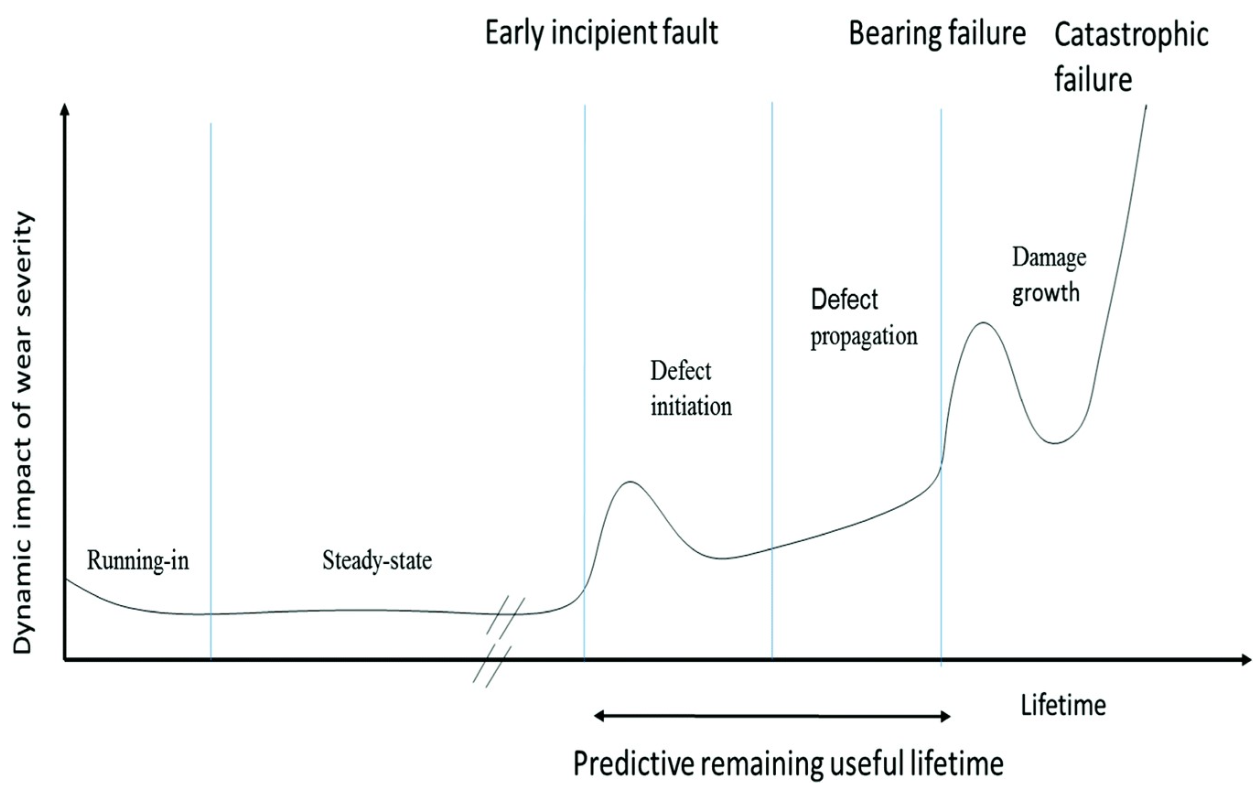
\includegraphics[width=0.7\linewidth]{assets/Screenshot 2026-01-20 at 11.57.41.png}
    \caption{Predictive Maintenence RUL}\label{fig:09-rul}
\end{figure}

%
\subsection{Manutenzione Predittiva in Applicazione alla Robotica}
L'obiettivo è monitorare la tensione della cinghia di trasmissione dei giunti del robot analizzando l'assorbimento di corrente.
%
\paragraph{Problema} Le cinghie possono essere tese in modo errato (troppo, troppo poco, o corretto).
%
\paragraph{Acquisizione Dati} Si monitora la corrente a 500Hz. Sono state definite 5 classi di tensione: Classe 0 $ = $ rischio rottura, Classi da 2 a 4 $ = $ condizioni OK. Vedi figura \ref{fig:09-dat}.
%
\paragraph{Data Management} I dati grezzi (troppi per il real-time) vengono aggregati in 14 feature (media, deviazione standard, skewness, kurtosis \dots) su 24 segmenti temporali. Vedi figura \ref{fig:09-500hz}.
%
\paragraph{Modello Analitico} Utilizza un algoritmo di Random Forest (\emph{Machine Learning}) per classificare il segnale in una delle 5 classi. I segmenti più critici del ciclo (fasi 10 e 11) sono quelli usati per calcolare il RUL basandosi sulla deviazione dalla distribuzione Gaussiana corretta. Vedi figure \ref{fig:09-rul}, \ref{fig:09-model}.
%
\paragraph{Architettura} Il training del modello avviene in Cloud, mentre la classificazione è eseguita a livello di Gateway (Edge). Vedi figura \ref{fig:09-arc}.

\begin{figure}
    \centering
    \begin{subfigure}{0.7\linewidth}
        \centering
        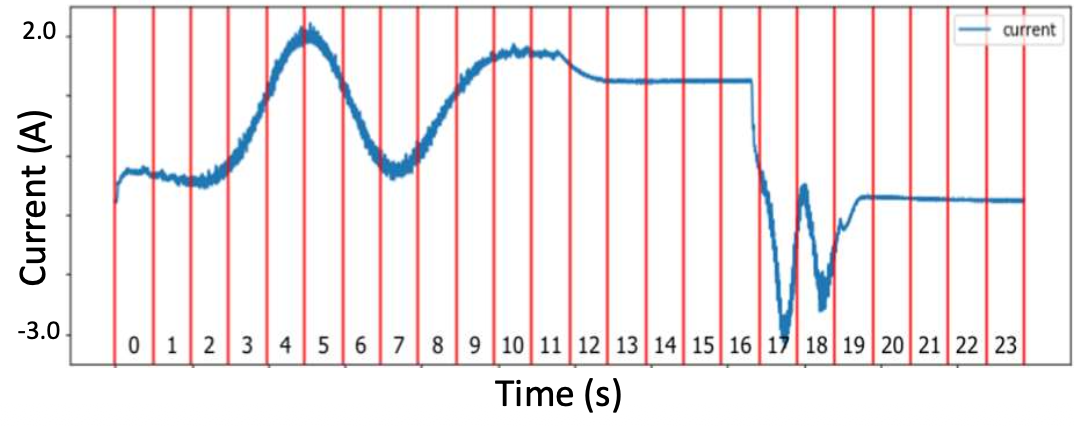
\includegraphics[width=\linewidth]{assets/Screenshot 2026-01-20 at 12.04.18.png}
        \caption{500Hz of Sample Graph}\label{fig:09-500hz}
    \end{subfigure}
    \begin{subfigure}{0.45\linewidth}
        \centering
        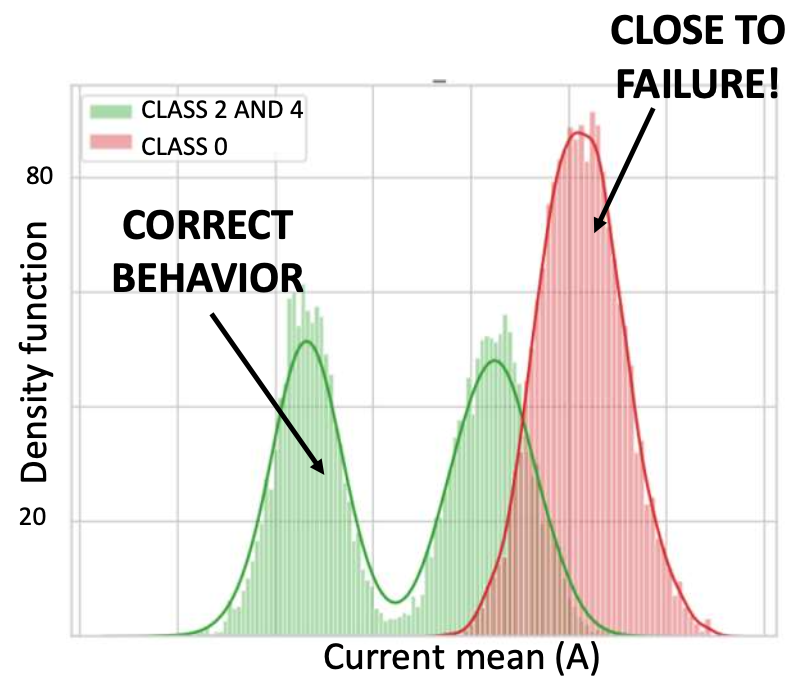
\includegraphics[width=\linewidth]{assets/Screenshot 2026-01-20 at 12.05.08.png}
        \caption{RUL Estimation}\label{fig:09-rul}
    \end{subfigure}
    \begin{subfigure}{0.5\linewidth}
        \centering
        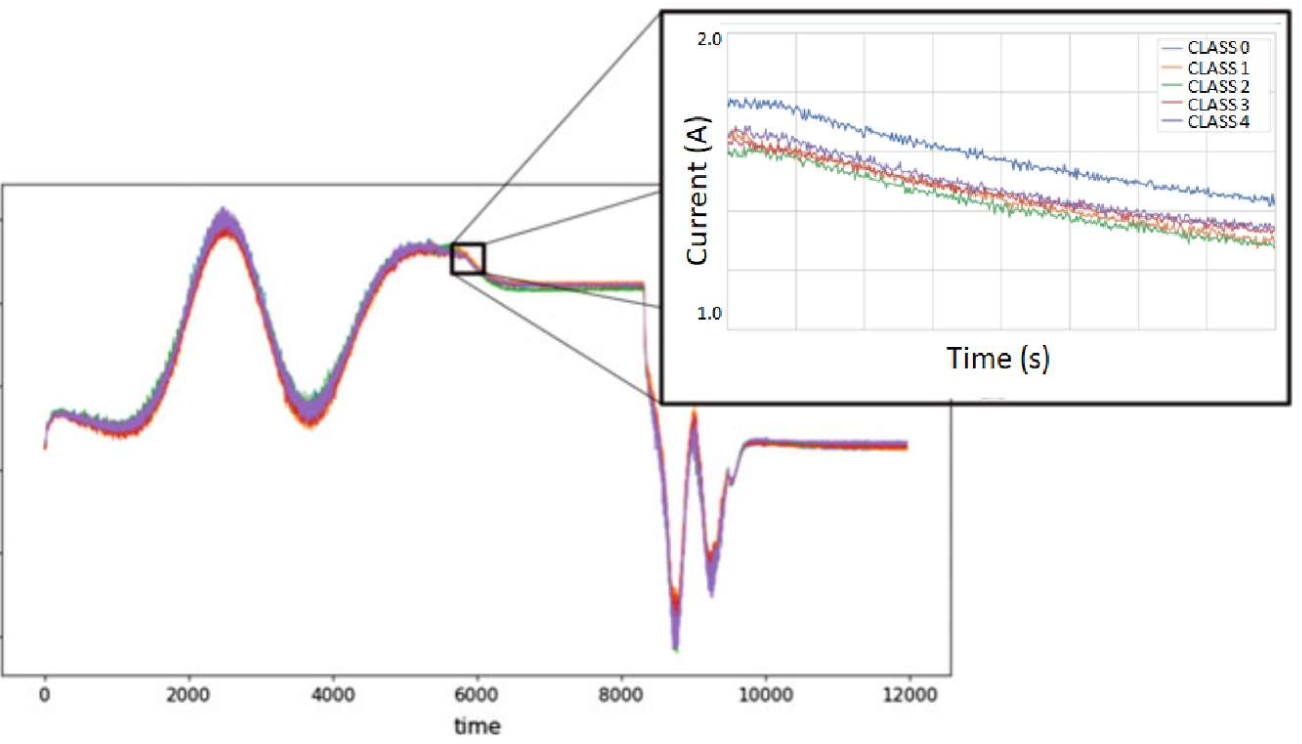
\includegraphics[width=\linewidth]{assets/Screenshot 2026-01-20 at 12.07.18.png}
        \caption{Data Acquisition}\label{fig:09-dat}
    \end{subfigure}
    \begin{subfigure}{0.45\linewidth}
        \centering
        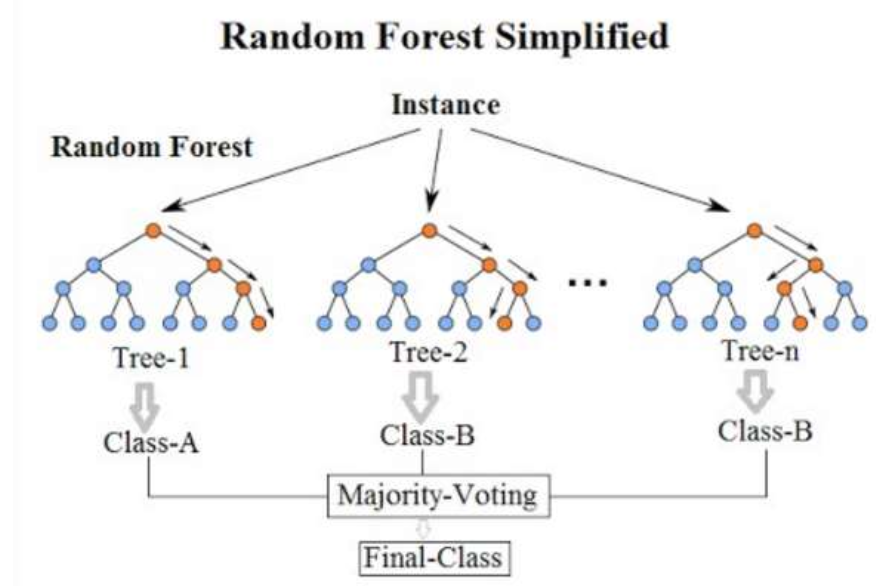
\includegraphics[width=\linewidth]{assets/Screenshot 2026-01-20 at 12.08.42.png}
        \caption{Predictive Model}\label{fig:09-model}
    \end{subfigure}
    \begin{subfigure}{0.45\linewidth}
        \centering
        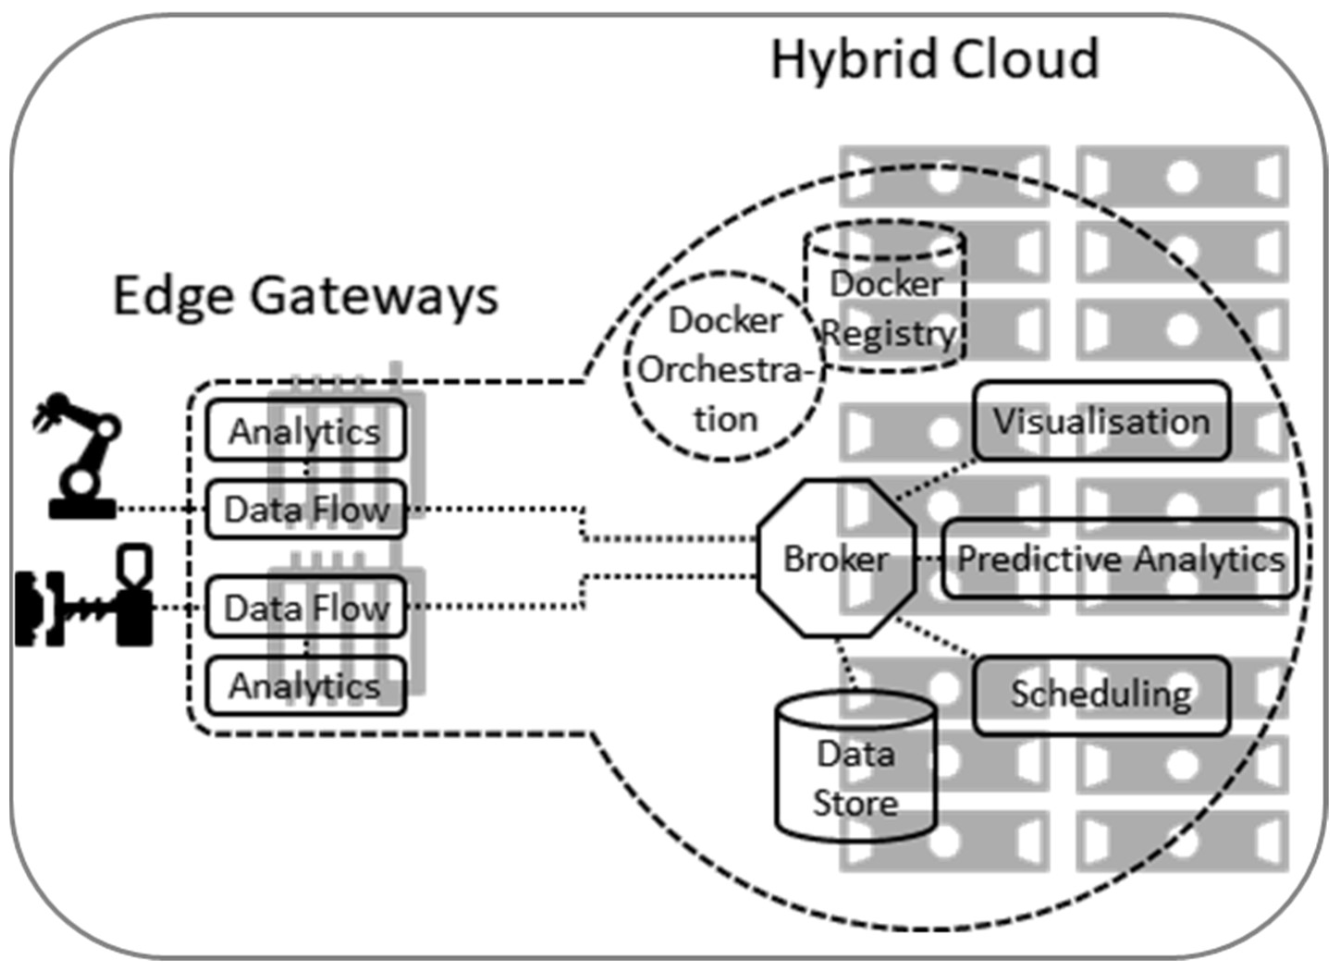
\includegraphics[width=\linewidth]{assets/Screenshot 2026-01-20 at 12.11.14.png}
        \caption{Edge Arc.}\label{fig:09-arc}
    \end{subfigure}
    \caption{}\label{fig:}
\end{figure}

%
\subsubsection{RUL Estimation}
Il calcolo per la stima del RUL è:
\[
    RUL(t)=\frac{1}{N_{t}} \sum_{x}^{X(t)}{(100-DEG(t))\prod_{s}^{S}P(x_{s} \in K(X_{s}(t_{0})))}
\]
Nell'equazione troviamo:
\begin{itemize}
    \item $ DEG(t) $: Stima di degrado come misura di errore percentuale.
\end{itemize}

%
\subsection{Manutenzione Predittiva in Applicazione alla Produzione di Ascensori}
Riguarda il monitoraggio di punzonatrici e piegatrici per evitare difetti dovuti all'usura dei cuscinetti.
%
\paragraph{Acquisizione Dati} Uso di accelerometri per monitorare vibrazioni e rumore.
%
\paragraph{Analisi del segnale} Ogni difetto (anello interno, esterno, sfera) genera frequenze specifiche: si applica l'Analisi di Inviluppo (Envelope Analysis) per isolare il rumore impulsivo generato dal difetto dalle frequenze naturali della macchina.
%
\paragraph{Edge Computing} Un Raspberry Pi esegue il calcolo delle frequenze di guasto e l'analisi di inviluppo localmente per ridurre la latenza, inviando poi al cloud solo i dati elaborati.

%
\section{Architettura IoT e Servizi Cloud}
L'infrastruttura proposta (progetto \emph{SERENA}) è ibrida e comprende:
\begin{enumerate}
    \item Edge Device: Raccoglie ed elabora i dati (es. feature extraction) quasi in tempo reale;
    \item Cloud: Centralizza lo storico dati, allena gli algoritmi di AI e ospita i servizi;
    \item Servizi, tra cui:
          \begin{itemize}
              \item Scheduling della Manutenzione: Pianifica gli interventi ottimizzando i costi e scegliendo il team adatto (es. esperto vs apprendista);
              \item Realtà Aumentata (AR e VR): Guide interattive e visualizzazioni 3D per assistere gli operatori durante le riparazioni, riducendo errori umani;
              \item Dashboard Analitiche: Visualizzazione dello stato di degrado e allarmi.
          \end{itemize}
\end{enumerate}

%
\section{Digital Twin nella Manutenzione}
Infine integriamo la manutenzione predittiva nel concetto di Digital Twin: ricordiamoci che il Digital Twin abilita un ciclo continuo di ottimizzazione che copre tutte le fasi, dal design alla dismissione (Retire phase), con la manutenzione predittiva che gioca un ruolo chiave nella fase produttiva.
